\documentclass[9pt, landscape, a4paper]{article}

\usepackage{fontspec}
\renewcommand{\normalsize}{\fontsize{9}{11}\selectfont}
\usepackage[english]{babel}
\babelfont{rm}{Noto Sans}
\babelfont{sf}{Noto Sans}

\usepackage{amsmath}
\usepackage{amssymb}
\usepackage{hyperref}
\usepackage{url}
\usepackage{graphicx}
\usepackage{geometry}
\usepackage{enumitem}
\usepackage{parskip}
\usepackage{chemfig}
\usepackage{pdfpages}
\usepackage{xcolor}
\usepackage{tikz}
\usepackage{fancybox}
\usepackage{makecell}
\usepackage{pgfplots}
\usepackage{ulem}
\usepackage{wrapfig}
\usepackage{subcaption}
\usepackage{esvect}
\usepackage{siunitx}
\usepackage{mathtools}
\usepackage{varwidth}
\usepackage{multicol}
\usepackage{titlesec}
\usepackage{bm}
\usepackage{forest}
\usepackage{upgreek}
\usepackage{tabularx}

\usetikzlibrary{arrows, arrows.meta}
\usetikzlibrary{decorations.pathreplacing}
\usetikzlibrary{patterns}
\pgfplotsset{compat=1.18}
\definecolor{darkgreen}{rgb}{0.0, 0.6, 0.0}
\DeclareMathOperator\arctanh{arctanh}

% ============= GEOMETRY =============
\geometry{
    a4paper,
    landscape,
    left=0.5cm,
    right=0.5cm,
    top=1.5cm, 
    bottom=0.5cm,
    footskip=0cm
}

\setlist{nosep, leftmargin=*}

\AtBeginDocument{
  \setlength{\abovedisplayskip}{3pt}
  \setlength{\belowdisplayskip}{3pt}
  \setlength{\abovedisplayshortskip}{0pt}
  \setlength{\belowdisplayshortskip}{0pt}
}

% ============= HEADER & TITLES =============
\usepackage{fancyhdr}
\pagestyle{fancy}
\fancyhf{}
\rhead{\small \vspace*{.1cm}Fluid Dynamics Cheatsheet}
\lhead{\small \vspace*{.1cm}Matteo Frongillo}
\cfoot{\small \vspace*{.4cm}\thepage}
\newcommand{\TotalPages}{12}
\cfoot{\small \vspace*{.4cm}\thepage/\TotalPages}
\renewcommand{\headrulewidth}{0pt}
\setlength{\headsep}{4pt}

\titlespacing*{\part}{0pt}{6pt}{1pt}
\titlespacing*{\section}{0pt}{6pt}{1pt}
\titlespacing*{\subsection}{0pt}{6pt}{1pt}
\titlespacing*{\subsubsection}{0pt}{6pt}{1pt}

\titleformat{\part}{\large\bfseries\color{black}}{\thepart.}{0.5em}{}
\titleformat{\section}{\bfseries\color{red!80}}{\thesection.}{0.5em}{}
\titleformat{\subsection}{\small\bfseries\color[HTML]{007AFF}}{\thesubsection}{0.5em}{}
\titleformat{\subsubsection}{\small\bfseries\color[HTML]{007355}}{\thesubsubsection}{0.5em}{}

% ============= META DATA =============
\newcommand{\pdftitle}[1]{\hypersetup{
  colorlinks=true,
  linkcolor=black,
  urlcolor=blue,
  pdftitle={#1},
  pdfauthor={Matteo Frongillo}
}}

% ============= RENEW COMMANDS =============

\makeatletter
\renewcommand{\author}[1]{%
  \def\@author{%
    #1\\
    \parbox{\textwidth}{%
      \centering
      \small Last update: \today
    }
  }%
}
\makeatother

\let\emptyset\varnothing

\makeatletter
\pgfmathdeclarefunction{arctan}{1}{%
    \begingroup
    \pgfmathparse{rad(atan(#1))}%
    \endgroup
}
\makeatother

\renewcommand{\tau}{\uptau}
\renewcommand{\nu}{\upnu}

% ============= NEW COMMANDS =============

\newcommand{\figbox}[1]{ 
  \begin{center}
    \fbox{\begin{varwidth}{\textwidth} #1 \end{varwidth}} 
  \end{center}       
}

\newcommand{\wrapfill}{
    \par
    \ifnum \value{WF@wrappedlines} > 0
        \addtocounter{WF@wrappedlines}{-1}%
        \null\vspace{
            \arabic{WF@wrappedlines}
            \baselineskip
        }
        \WFclear
    \fi
    \phantom{}
}

\ExplSyntaxOn
\DeclareDocumentCommand{\integral}{d[] d[] d[] d[]}
{
    \IfNoValueTF{#3}{
        \IfNoValueTF{#4}{
            \displaystyle \int #1\,d#2
        }{
            \text{Error: either 2 or 4 arguments must be provided}
        }
    }{
        \IfNoValueTF{#4}{
            \text{Error: either 2 or 4 arguments must be provided}
        }{
            \displaystyle
            \int\limits
                \IfNoValueF{#1}{\c_math_subscript_token{#1}}
                ^{\IfNoValueTF{#2}{}{#2}}
                #3\, d#4
        }
    }
}
\ExplSyntaxOff

\newcommand*\circled[1]{\tikz[baseline=(char.base)]{
            \node[shape=circle,draw,inner sep=1pt] (char) {\small #1};}}

\makeatletter
\newcommand*{\rom}[1]{\expandafter\@slowromancap\romannumeral #1@}
\makeatother

\makeatletter
\newcommand{\shorteq}{\mathrel{\mkern0.2mu\mathpalette\shorteq@\relax\mkern0.2mu}}
\newcommand{\shorteq@}[2]{\scalebox{0.5}[1]{$\m@th#1=$}}

\newcommand{\longeq}[1]{\mathrel{\mathpalette\longeq@{#1}}}
\newcommand{\longeq@}[2]{%
  \begingroup
  \sbox\z@{$\m@th#1=$}%
  \ifdim#2<\wd\z@
    \resizebox{#2}{\height}{\box\z@}%
  \else
    \ifdim#2<3\wd\z@
      \hbox to #2{$\m@th#1=\hss=\hss=\hss=$}%
    \else
      \hbox to #2{$\m@th#1=\cleaders\hbox to 0.2\wd\z@{\hss$#1=$\hss}\hfil=$}%
    \fi
  \fi
  \endgroup
}
\makeatother

\newcommand{\const}{%
  \ \mathrel{\ooalign{%
    \hfil$c$\hfil\cr
    \hfil\kern0.10em\raisebox{-0.4ex}{\rule{0.08pt}{1.7ex}}\hfil\cr
  }}%
}

\DeclareMathOperator{\rot}{rot}

\newcommand{\difference}{\,\backslash\,}
\newcommand{\rem}{\underline{Remark}: }
\newcommand{\nots}{\underline{Notation}: }
\newcommand{\note}{\underline{Note}: }
\newcommand{\prf}{\underline{Proof}: }
\newcommand{\exs}{\underline{Example}: }
\newcommand{\defs}{\underline{Definition}: }
\newcommand{\wrn}{\underline{Warning}: }
\newcommand{\sht}{\ |\ }
\newcommand{\pph}[1]{\paragraph{#1} \phantom{}\\}
\newcommand{\dm}{\displaystyle}
\newcommand{\rad}{^{\mathrm{c}}}
\newcommand{\dsum}[2]{\displaystyle \sum_{#1}^{#2}}
\newcommand{\dx}[2]{\dfrac{{\mathrm{d}}^{#1}{#2}}{\mathrm{d}x^{#1}}}
\newcommand{\der}[2]{\dfrac{{\mathrm{d}}{#1}}{\mathrm{d}{#2}}}
\newcommand{\cel}{$^\circ$C}

% ============= DOCUMENT CONTENT =============

\begin{document}
\pdftitle{Fluid dynamics}
\vspace*{-.5cm}
\setlength{\columnsep}{0.5cm}

\begin{multicols*}{3}
\raggedcolumns
\vspace*{-.5cm}
\part{Viscous flow}
\section*{Symbology}
{\scriptsize
\renewcommand{\arraystretch}{1.5}
\begin{tabular}{clc|clc}
  \textbf{Symb} & \makecell{\textbf{Name}} & \textbf{Units} & \textbf{Symb} & \makecell{\textbf{Name}} & \textbf{Units} \\
    $\nu$ & Kinematic viscosity & m$^2$/s & $\eta$ & Dynamic viscosity & Pa$\cdot$s \\
    $\tau$ & Shear stress & Pa & $dn$ & Normal distance & m \\
    $du/dy$ & Rate of strain & [-] & $e_{\, \text{Diss}}$ & Spec. diss. power & W/m$^3$\\
\end{tabular}}

\section{Flows with friction}
\begin{center}
  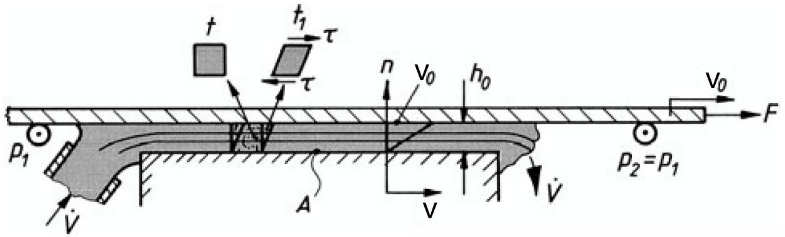
\includegraphics[width=.85\linewidth]{media/smallgap.png}
\end{center}
\[F = \eta\dfrac{v_0\cdot A}{h_0} \Longrightarrow \tau = \dfrac{F}{A} = \eta\dfrac{v_0}{h_0} = \eta\dfrac{dv}{dn}\]

For pipes:
\[F_\tau = \tau A \Longrightarrow M_\tau = F_\tau y = \tau \cdot l \cdot 2\pi r_0^2\]

\subsection{Friction law}
\begin{equation*}
  \tau = -\eta \dfrac{dv}{dn}\quad ; \quad \dot{e}_{\, \text{Diss}} = \eta\left(\dfrac{dv}{dn}\right)^2
\end{equation*}

\section{Viscosity}
If $\eta = 0$, the fluid is called inviscid.\\[2pt]
No slip condition: velocity of a particle closest to the wall has
velocity equal to the wall velocity.

\subsection{Reynolds Number}
\begin{gather*}
    Re = \dfrac{\rho v L}{\eta} = \dfrac{v L}{\nu}\quad ; \quad \nu = \dfrac{\eta}{\rho}
\end{gather*}

\subsection{Newtonian fluids}
\begin{itemize}
  \item Rate of deformation $\mathrm{d}u / \mathrm{d}y$ (velocity gradient) is linearly proportional to the shear stress $\tau$
  \item The constant of proportionality is the viscosity (slope)
  \item $\dm \eta = \frac{\tau}{\mathrm{d}u / \mathrm{d}y} =$ constant
\end{itemize}

\subsection{Non-Newtonian fluids}
Non-linear relation between shear stress and deformation rate due
to non-constant viscosity.
\[\tau = \eta\left(\frac{\partial u}{\partial y}\right) \cdot \frac{\partial u}{\partial y}\]

\subsubsection{Dilatant (shear thickening) fluids}
Viscosity increases with increasing strain rate.

\subsubsection{Plastic or pseudo-plastic (shear thinning) fluids}
Viscosity decreases with increasing strain rate.

\subsubsection{Bingham medium}
Flow occurs only after a yield stress $\tau_0$ is reached.

\subsection{Graphical representation}
\begin{center}
  
\includegraphics[width=.7\linewidth]{media/viscosity.png}
\end{center}

\section{Flow profiles}
\subsection{Couette flow profiles (constant velocity gradient)}
\begin{minipage}{0.5\linewidth}
  \begin{gather*}
    \frac{\partial u(y)}{\partial y} = \frac{v_p}{s}\\
    e_{\, \text{Diss}} = \eta\left(\frac{\partial u(y)}{\partial y}\right)^2 = \eta\left(\frac{v_p}{s}\right)^2\\
    P_{\, \text{Diss}} = \int_V e_{\, \text{Diss}}(y)\ dV
  \end{gather*}
\end{minipage}%
\begin{minipage}{0.5\linewidth}
  \begin{center}
    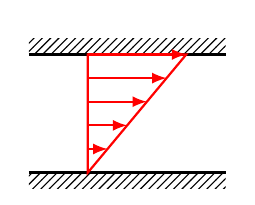
\begin{tikzpicture}[scale=.5][ht!]
      % Parameters
      \def\H{3}       % Distance between plates
      \def\W{5}       % Width of plates
      \def\xBase{1.5} % Base x-coordinate for the velocity profile
      \def\vMax{2.5}  % Maximum velocity vector length
  
      % Bottom stationary plate
      \fill[pattern=north east lines] (0,-0.4) rectangle (\W,0);
      \draw[thick] (0,0) -- (\W,0);
  
      % Top moving plate
      \fill[pattern=north east lines] (0,\H) rectangle (\W,\H+0.4);
      \draw[thick] (0,\H) -- (\W,\H);
  
      % Velocity profile envelope (triangle)
      \draw[red, thick] (\xBase,0) -- (\xBase,\H) -- (\xBase+\vMax,\H) -- cycle;
  
      % Velocity vectors
      \foreach \y in {0.6, 1.2, 1.8, 2.4, 3.0} {
          \pgfmathsetmacro{\xEnd}{\xBase + \y*(\vMax/\H)}
          \draw[-{latex[length=2.5mm]}, red, thick] (\xBase,\y) -- (\xEnd,\y);
      }
    \end{tikzpicture}
  \end{center}
\end{minipage}

\subsection{Poiseuille flow profiles (parabolic velocity gradient)}
\begin{minipage}{0.5\linewidth}
  \begin{align*}
    &\frac{\partial u(y)}{\partial y} = \frac{4 v_{\text{max}}}{s} \left(1 - \frac{2y}{s}\right) \\
    &v(r) = ar^2 + br + c \\
    &e_{\, \text{Diss}} = \eta \frac{16 v_{\text{max}}^2}{s^2} \left(1 - \frac{2y}{s}\right)^2 \\
    &P_{\, \text{Diss}} = \frac{16 \eta A v_{\text{max}}^2}{3s}
  \end{align*}
\end{minipage}%
\begin{minipage}{0.5\linewidth}
  \begin{center}
    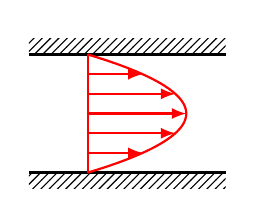
\begin{tikzpicture}[scale=.5]
      % Parameters
      \def\H{3}       % Distance between plates
      \def\W{5}       % Width of plates
      \def\xBase{1.5} % Base x-coordinate for the velocity profile
      \def\vMax{2.5}  % Maximum velocity vector length

      % Bottom stationary plate
      \fill[pattern=north east lines] (0,-0.4) rectangle (\W,0);
      \draw[thick] (0,0) -- (\W,0);

      % Top stationary plate
      \fill[pattern=north east lines] (0,\H) rectangle (\W,\H+0.4);
      \draw[thick] (0,\H) -- (\W,\H);

      % Velocity profile envelope (parabola)
      \draw[red, thick] (\xBase,0) -- (\xBase,\H);
      \draw[red, thick, domain=0:\H, samples=50] plot ({\xBase + 4*\vMax*(\x/\H)*(1-\x/\H)}, \x);

      % Velocity vectors
      \foreach \y in {0.5, 1.0, 1.5, 2.0, 2.5} {
          \pgfmathsetmacro{\v}{4*\vMax*(\y/\H)*(1-\y/\H)}
          \pgfmathsetmacro{\xEnd}{\xBase + \v}
          \draw[-{latex[length=2.5mm]}, red, thick] (\xBase,\y) -- (\xEnd,\y);
      }
    \end{tikzpicture}
  \end{center}
\end{minipage}

\section{Laminar pipe flow}
\subsection{$p_1 > p_2$}
\[\frac{\partial p}{\partial z} = \frac{p_2 - p_1}{L}\]

\subsection{Constant linear flow profiles}
\[\dot{V} = v_m A = v_m R^2 \pi\]

\subsection{Parabolic flow profiles}
\begin{gather*}
  \dot{V} = \integral[v(r)][A] = \dfrac{v_{max}\cdot R^2\pi}{2}\\
  v(r) = v_{max}\left(1-\dfrac{r^2}{R^2}\right)\\
  \dfrac{dv}{dr} = -2v_{max}\dfrac{r}{R^2}\\
  P_{\, \text{Diss}} = \integral[0][L][\integral[0][2\pi][\integral[0][R][\eta\left(-2v_{max}\dfrac{r^2}{R^2}\right)\cdot r][r]][\varphi]][x]\\
  P_{\, \text{Diss}} = 2\pi L \integral[0][R][\eta\left(-2v_{max}\dfrac{r^2}{R^2}\right)\cdot r][r] = 2\pi L\eta v_{max}^2 = 8\pi L\eta v_{m}^2
\end{gather*}

\section{Flows in gaps and bearings}
\subsection{Assumptions in gaps and bearings}
\begin{minipage}[t]{0.5\linewidth}
  \begin{itemize}
    \item Newtonian fluid with\\constant viscosity $\eta$
    \item Incompressible fluid
    \item Very low Reynolds\\number $Re < 2000$
    \item Laminar flow
  \end{itemize}
  \end{minipage}%
\begin{minipage}[t]{0.5\linewidth}
  \begin{itemize}
    \item Balance of pressure and\\viscous forces
    \item No slip condition at the walls
    \item No acceleration (negligible)
    \item Pressure is uniform across the thickness $\partial p/\partial y \approx 0$
  \end{itemize}
\end{minipage}

\subsection{Equilibrium of forces}
\begin{gather*}
  \sum F_x = 0 \Longrightarrow pA_p - (p+dp)A_p + \tau A_\tau + (\tau + d\tau)A_\tau = 0\\
  A_p = dy \cdot b\quad ; \quad A_\tau = dx \cdot b \quad ; \quad \tau = \eta \dfrac{dv}{dy} \rightarrow \dfrac{d\tau}{dy}\\
  \boxed{\eta\dfrac{d^2v(x,y)}{dy^2} = \dfrac{dp(x)}{dx} = p'}
\end{gather*}

\subsection{Basic velocity equation}
\[v(x,y) = \frac{1}{\eta} \cdot p' \cdot \frac{y^2}{2} + c(x)y + d(x)\]

\subsubsection{Gap flow (walls not moving)}
\begin{minipage}{0.5\linewidth}
  \begin{align*}
    &v(x,y) = \dfrac{p'(x)}{2\eta}\left[y^2-h(x)y\right]\\
    &c(x) = -\dfrac{h(x)}{2\eta} \cdot \dfrac{dp(x)}{dx}\\
    &d(x) = 0
  \end{align*}
\end{minipage}%
\begin{minipage}{0.5\linewidth}
\begin{center}
  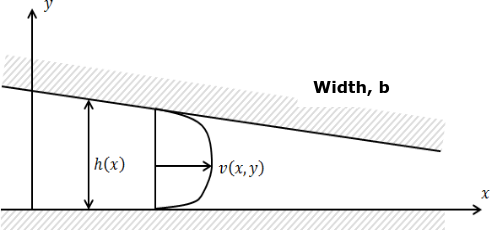
\includegraphics[width=\linewidth]{media/gapflow.png}
\end{center}
\end{minipage}
\vfill\phantom{}
\newcolumn

\subsubsection{Plain bearing / Creeping gap flow (one wall moving)}
\begin{center}
  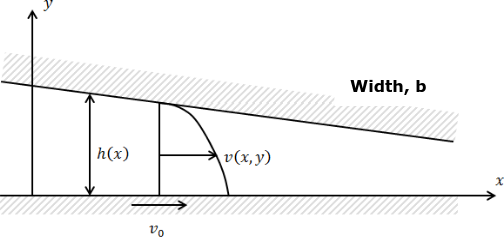
\includegraphics[width=.4\linewidth]{media/bearingflow.png}
\end{center}
Assumption for $Re \ll 1$: $\eta \dfrac{d^2v}{dy^2}=\dfrac{dp}{dx}=p'$
\begin{align*}
  &v(x,y) = \dfrac{p'(x)}{2\eta}\left[y^2-h(x)y\right] + \dfrac{v_0}{h(x)}\left[h(x)-y\right]\\
  &c(x) = -\dfrac{h(x)}{2\eta} \cdot \dfrac{dp(x)}{dx} - \dfrac{v_0}{h(x)}\\
  &d(x) = v_0
\end{align*}

For the simplest, parabolic velocity profile case:
\begin{gather*}
  h(x)=h_0\quad ; \quad v_0 = 0\quad ; \quad p' = \dfrac{dp(x)}{dx} = \dfrac{\Delta p}{\Delta L} = -\dfrac{12\eta v_m}{h_0^2}\\
  v(y) = \dfrac{p'}{2\eta}\left(y^2-h_0y\right) \Longrightarrow \dfrac{\partial v}{\partial y} = 0 = \dfrac{p'}{2\eta}\left(2y-h_0\right)\\
  y = \dfrac{h_0}{2} \Longrightarrow v_{max} = v\left(y=\dfrac{h_0}{2}\right) = -\dfrac{h_0^2p'}{8\eta} = \dfrac{3}{2}v_m\\
  v_m = -\dfrac{\Delta p \cdot h_0^2}{12\eta L}\\
  \dot{V} = b\integral[0][h_0][v(y)][y] = -b\dfrac{p'h_0^3}{12\eta} = \dfrac{h_0^2}{6\eta}b\Delta p
\end{gather*}

General sliding bearings:
\begin{gather*}
  \dot{V} = b\integral[0][h(x)][\dfrac{p'}{2}\eta\left(y^2-h(x)y\right) + \dfrac{v_0}{h(x)}\left(h(x)-y\right)][y]\\
  \dot{V} = -b\dfrac{p'h^3_{(x)}}{12\eta} + b\dfrac{v_0h(x)}{2} = \const\\
  p' = 6\eta v_0\left(\dfrac{1}{h(x)^2}-\dfrac{\dot{V}}{bh(x)^3}\right)
\end{gather*}

\subsubsection{General form of the volumetric flow rate}
\begin{gather*}
  v(x,y) = \dfrac{1}{\eta}p'\dfrac{y^2}{2}+c(x)+d(x)\\
  \dot{V} = b\integral[0][h(x)][v(x,y)][y] = b\left[-\dfrac{h^3(x)}{6\eta}p' + c(x)\dfrac{h^2(x)}{2} + d(x)h(x)\right] = \const\\
  p' = \dfrac{6\eta}{h(x)^3}\left(\dfrac{\dot{V}}{b}-c(x)\dfrac{h(x)^2}{2} - d(x)h(x)\right)
\end{gather*}

\subsubsection{Possible semplifications}
If h $\ll$ D:
\[A = \int_A r\ dr\ d\varphi \approx \pi D h\]

\subsection{Specific dissipation power}
\begin{gather*}
  P = \tau A v = \eta \frac{\partial v}{\partial n} A v \quad ; \quad dP = dFdv\\
  dF_\tau = d\tau dA = \eta \frac{dv}{dy} dxdz\\
  e_{\, \text{Diss}} = \frac{dP_\tau}{dV} = \frac{\eta\frac{dv}{dy}dxdzdv}{dxdydz} = \eta\left(\frac{dv}{dy}\right)^2 = \eta\left(\frac{\partial v}{\partial y}\right)^2\\
  P_{\, \text{Diss}} = \int_V \!\!e_{\, \text{Diss}}\ dV = \iiint_V \!\!e_{\, \text{Diss}}\ dxdydz = M \cdot \omega
\end{gather*}

\subsubsection{Pressure loss according to Bernoulli}
\[p_1 - p_2 = \rho\frac{P_{\, \text{Diss}}}{\dot{m}} = \frac{P_{\, \text{Diss}}}{\dot{V}} = \frac{8\pi L \eta v_m}{R^2} \left(= \rho g h\right)\]

\part{Boundary layers}
{\scriptsize
\newcommand{\rowstrut}{\rule{0pt}{4ex}}
\begin{tabular}{clc|clc}
  \textbf{Symb} & \makecell{\textbf{Name}} & \textbf{Units} & \textbf{Symb} & \makecell{\textbf{Name}} & \textbf{Units}\\[-1ex]
  \rowstrut $v_\infty$ & \makecell[l]{free-stream\\velocity} & m/s & $v(y)$ & \makecell[l]{local velocity in\\boundary layer} & m/s\\
  \rowstrut $\delta$ & \makecell[l]{boundary layer\\thickness} & m & $\delta^*$ & \makecell[l]{BL displacement\\thickness} & m\\
  \rowstrut $\theta$ & \makecell[l]{momentum\\thickness} & m & $\tau_w$ & \makecell[l]{wall shear stress} & Pa\\
  \rowstrut $\nu$ & \makecell[l]{kinematic\\viscosity} & m$^2$/s & $\eta$ & \makecell[l]{dynamic\\viscosity} & Pa$\cdot$s\\
  \rowstrut $Re_x$ & \makecell[l]{Reynolds num.\\at position $x$} & -- & $\dot{V}_{BL}$ & \makecell[l]{boundary-layer\\volume flow rate} & m$^2$/s
\end{tabular}}

Boundary layers develop due to wall shear stress $\tau$ and fluid viscosity $\nu$.

\section{Laminar vs. Turbulent boundary layers}
\subsection{Critical Reynolds number}
\begin{center}
  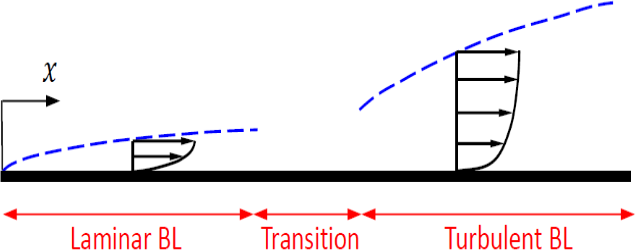
\includegraphics[width=.7\linewidth]{media/reynoldBL.png}
\end{center}

Reynolds number for the BL on a flat plate:
\[Re_x = \dfrac{v_\infty x}{\nu} = \dfrac{v_\infty \cdot l_{char}}{\nu}\]

$Re$ \textbf{increases} with the distance from the plate entry.\\
\textbf{Transition to turbulent}: $Re_x \geq 5\times 10^5$

\newcolumn
\subsection{Flat plate boundary layer}
\begin{center}
  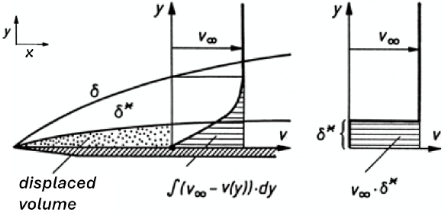
\includegraphics[width=.55\linewidth]{media/displacement_thickness.png}
\end{center}

\vspace*{-.4cm}
\begin{gather*}
  \delta(x) \approx \sqrt{x}\quad ; \quad \tau(x) \approx 1/\delta(x) = 1/\sqrt{x}\\
  \dot{V}_{BL} = v_\infty \cdot \delta^*(x)\\
  \text{with 2 plates: }\dot{V}_{BL} = A^*\cdot v = \left(\dfrac{d - 2\delta^*}{2}\right)\pi \cdot v
\end{gather*}

\subsection{Turbolent BL}
\subsubsection{Non-dimensional forms}
Non-dimensional plot of wall normal turbulent velocity profile:
\begin{center}
  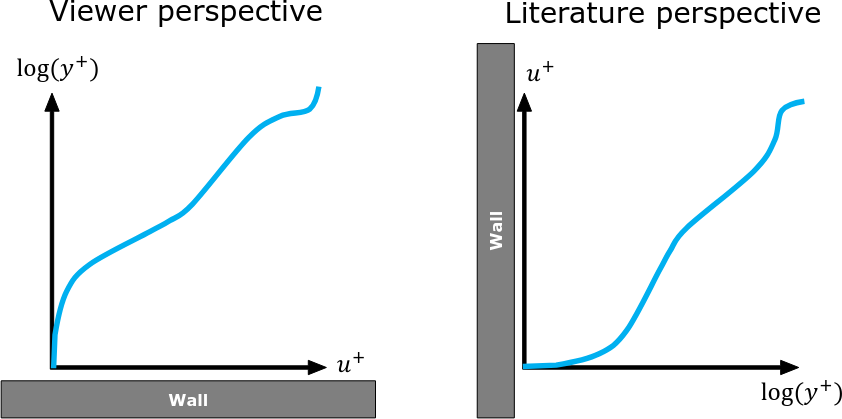
\includegraphics[width=.7\linewidth]{media/turbolent_BL.png}
\end{center}
\begin{itemize}
  \item Friction velocity: $u_\tau = \sqrt{\dfrac{\tau_\text{wall}}{\rho}}$
  \item Dimensionless wall parallel velocity: $u^+ = \dfrac{u}{u_\tau}$
  \item Dimensionless wall distance: $y^+ = \dfrac{yu_\tau}{\nu}$
\end{itemize}

\subsection{Rough and smooth walls and the effect on friction}
\subsubsection{No-slip condition}
\begin{center}
  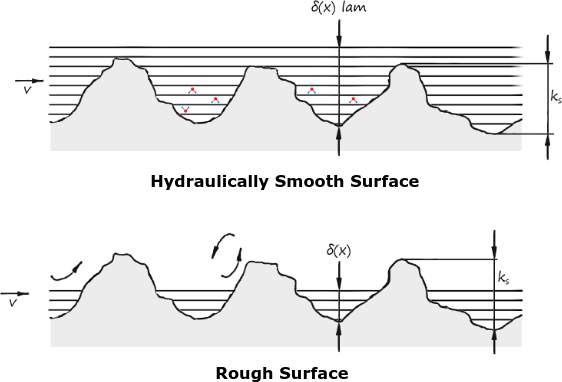
\includegraphics[width=.7\linewidth]{media/noslip.png}
\end{center}
\begin{itemize}
  \item Hydraulically smooth surface: $\delta(x) > k_s$
  \item Rough surface: $\delta(x) < k_s$. Leads to vortex.
\end{itemize}

\newcolumn
\section{Flow separation}
\subsection{Flow separation conditions}
\begin{enumerate}
  \item Friction
  \item Pressure increase
\end{enumerate}

At sharp edges, the flow always separate.

\subsection{Pressure gradient}
\begin{center}
  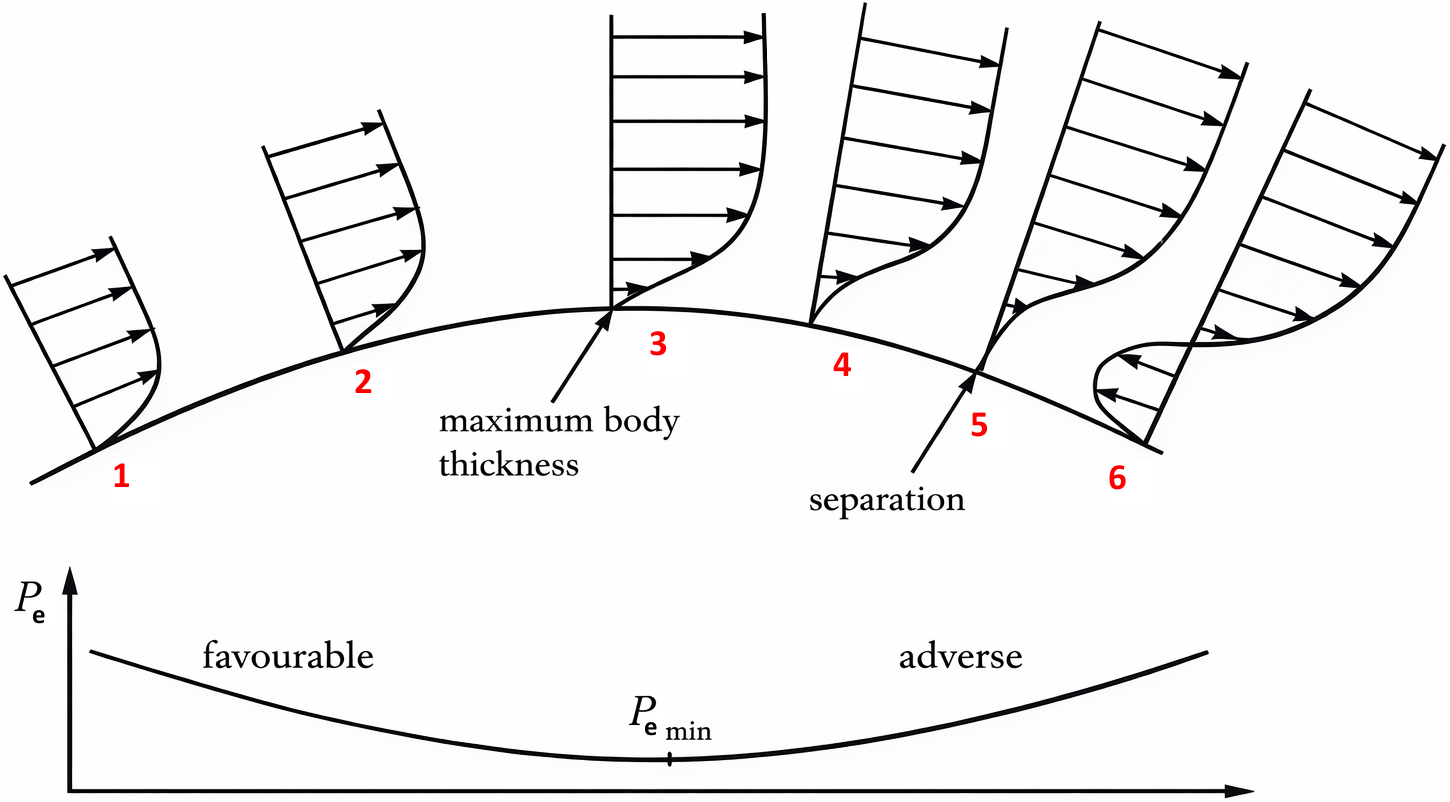
\includegraphics[width=.7\linewidth]{media/flow_separation.png}
\end{center}

\subsubsection{Comparison of boundary layer profile shape}
Comparing BL as a function of the pressure gradient:
\[\dfrac{dP}{dx} \sim -\dfrac{dU(x)}{dx}\quad ; \quad \tau_\text{wall} = m\dfrac{dv}{dy_{y=0}}\]

\begin{enumerate}[label=\color{red}\textbf{\arabic*.}]
  \item favorable pressure gradient: $\dfrac{\partial p}{\partial x} \ll 0$\\[0ex]
  \item favorable pressure gradient: $\dfrac{\partial p}{\partial x} < 0$\\[0ex]
  \item zero pressure gradient: $\dfrac{\partial p}{\partial x} = 0$\\[0ex]
  \item mild adverse pressure gradient: $\dfrac{\partial p}{\partial x} > 0$\\[0ex]
  \item critical adverse pressure gradient: $\dfrac{\partial p}{\partial x} > 0, \tau_\text{wall} = 0$\\[0ex]
  \item large adverse pressure gradient: $\dfrac{\partial p}{\partial x} \gg 0$\\[0ex]
\end{enumerate}

\subsection{Flow separation gradients}
\begin{center}
  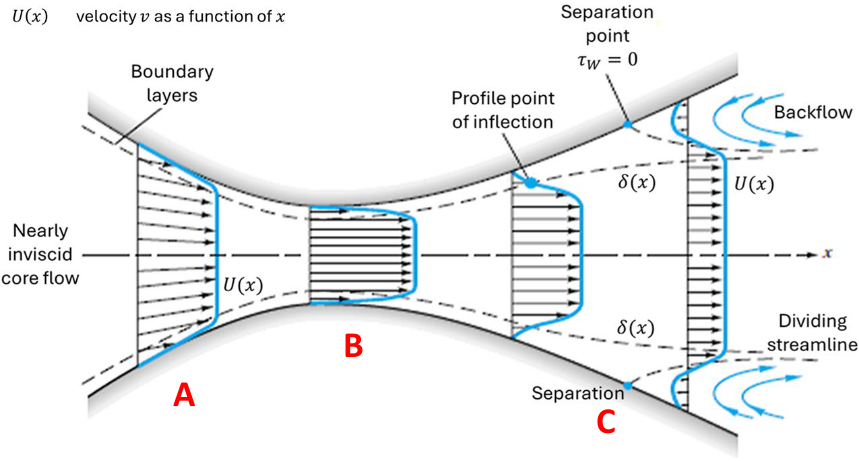
\includegraphics[width=.88\linewidth]{media/flow_gradients.png}
\end{center}

\newcolumn
\subsubsection{Nozzle (Favorable Pressure Gradient) {\color{red} (A)}}
\[\frac{dp}{dx} < 0\quad ; \quad \frac{dU}{dx} > 0\]
\begin{itemize}
  \item Decreasing pressure and decreasing area
  \item Pressure decreases in the flow direction
  \item Pressure force is in the flow direction
  \item No flow separation
\end{itemize}

\subsubsection{Throat {\color{red} (B)}}
\[\frac{dp}{dx} = 0 \quad ; \quad \frac{dU}{dx} = 0\]
\begin{itemize}
  \item Constant pressure and constant area
  \item Fluid particles in the BL slow down due to shear stress only
  \item No flow separation can occur
  \item Similar to a flat plate
\end{itemize}

\subsubsection{Diffuser (Adverse Pressure Gradient) {\color{red} (C)}}
\[\frac{dp}{dx} > 0 \quad ; \quad \frac{dU}{dx} < 0\]
\begin{itemize}
  \item Pressure increases in the flow direction
  \item Pressure force is in opposite direction of the flow
  \item \textbf{Back flow situation}: Fluid particles close to the wall with low momentum may come to a stop or even move in opposite direction of the main flow
\end{itemize}

\subsection{Influence of $Re$ on blunt bodies}
\begin{itemize}
  \item $Re < 1$: No vortex formation
  \item $Re \approx 10^5$: Laminar BL, vortex formation in dead water area 
  \item $Re > 10^6$: BL partially turbolent, vortex on the body surface
\end{itemize}

\part{Drag and Lift Forces}
\textbf{Drag force}: parallel and opposite to the relative flow direction\\
\textbf{Lift force}: perpendicular to the relative flow direction

\section{Drag force and drag coefficient}
\subsection{Drag force}
\figbox{$\dm F_D = C_D q_\infty A_P = C_D\frac{1}{2}\rho v_\infty^2 A_p$}

where:
\begin{gather*}
  C_D: \text{drag coefficient } (\mu)\quad ; \quad A_p: \text{project area}\\
  q_\infty: \text{dynamic contribution}
\end{gather*}

\subsubsection{Drag force and power on a body in a flow}
\figbox{$\dm F_D = F_P + F_\tau\quad ; \quad P_D = F_D v_\infty$}
\textbf{Friction drag}: friction forces $F_\tau$ due to wall shear stress $\tau_\text{wall}$\\
\textbf{Pressure drag}: pressure forces $F_P$ due to pressure variation along
the surface of the object

\subsection{Drag on smooth circular cylinders}
\subsubsection{Prandlt's experiment}
\begin{center}
  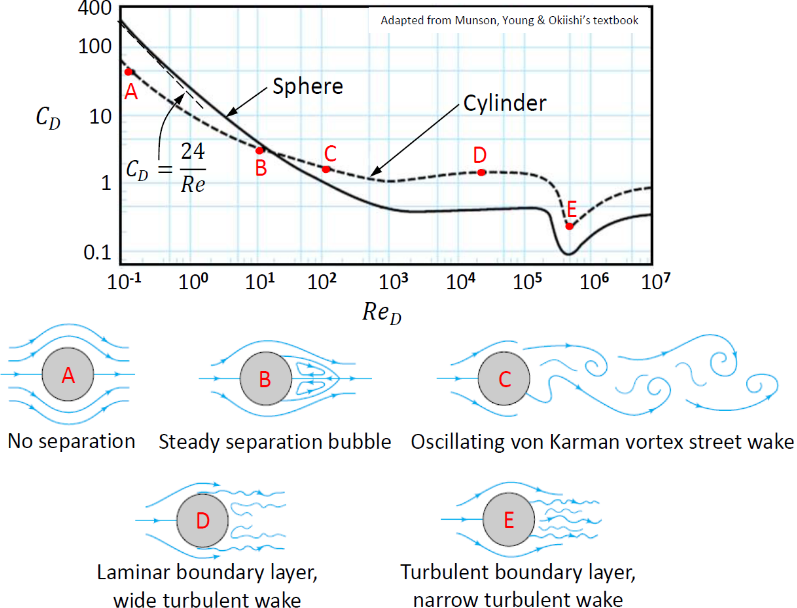
\includegraphics[width=.9\linewidth]{media/Stokes.png}
\end{center}
\subsubsection{Stokes formula and Stokes law}
\figbox{$F_D \approx F_\tau = 3\pi\eta dv_\infty \Longrightarrow C_D = \dfrac{24}{Re}$}
\vspace*{-.2cm}
\pph{Velocity of a sphere}
\vspace*{-.2cm}
\begin{gather*}
  \dfrac{1}{2}C_D\rho_\text{air}Av_\infty = \rho_\text{sph}V_\text{sph}g\quad ; \quad A = \left(\dfrac{d}{2}\right)^2\pi\quad ; \quad V = \left(\dfrac{d}{2}\right)^3\pi\\[.5ex]
  \boxed{v_\infty = \sqrt{\dfrac{4}{3}\dfrac{d\cdot g\cdot \rho_\text{sph}}{C_D \cdot \rho_\text{air}}}}
\end{gather*}

\subsubsection{Free falling sphere}
\begin{gather*}
  F_{res} = F_g - F_n \Longrightarrow F_g = F_n\\
  mg = C_D A \rho_\text{fluid} \dfrac{v_\infty^2}{2} \Longrightarrow v_\infty = \sqrt{\dfrac{2mg}{C_D A \rho_\text{fluid}}}
\end{gather*}

\pph{Velocity profile at the initial phase ($F_{res} \neq 0$)}
\begin{gather*}
  m\dfrac{dv}{dt} = mg - C_D A \rho_\text{fluid}\dfrac{v^2}{2}\\
  \integral[0][t][][t] = \integral[0][v][\dfrac{m}{mg - C_D A \rho_\text{fluid} \dfrac{v^2}{2}}][v]\\
  v(t) = v_\infty \tanh\dfrac{gt}{v_\infty}
\end{gather*}
\vfill

\pph{Duration of the initial phase}
If steady terminal velocity $v(t) = v_\infty \cdot 0.99$:
\begin{gather*}
  \tanh\dfrac{gt}{v_\infty} = 0.99 \Longrightarrow \dfrac{gt}{v_\infty} = \arctanh(0.99)\\[1ex]
  t = \dfrac{v_\infty \arctanh(0.99)}{g} = \dfrac{v_\infty \cdot 2.65}{g}
\end{gather*}

\subsection{Lift-induced drag and Parasitic drag}
\begin{gather*}
  C_D = C_{D_0} + C_{D_i}\\
  C_{D_i} = \dfrac{C_L^2}{\pi e AR}\quad ; \quad AR = \dfrac{b^2}{A}
\end{gather*}

\begin{itemize}
  \item low speed $\rightarrow$ induced drag dominates
  \item high speed $\rightarrow$ parasitic drag dominates
\end{itemize}

\subsubsection{Parasitic drag}
Drag not due to lift generation\\
(skin friction + form drag + interference drag).
\[
F_{D_0} = C_{D_0}\dfrac{1}{2}\rho v_\infty^2 A
\]

\subsubsection{Lift-induced drag}
Drag due to lift generation, caused by wing-tip vortices and downwash.
\[
F_{D_i} = C_{D_i}\dfrac{1}{2}\rho v_\infty^2 A
\]

For constant lift:
\[
F_{D_0} \sim v_\infty^2\quad ; \quad F_{D_i} \sim \dfrac{1}{v_\infty^2}
\]

\section{Lift force and lift coefficient}
\subsection{Angle of Attack (AOA)}
Variable angle between the chord line and the relative wind;
affects lift and can change during flight.
\begin{center}
  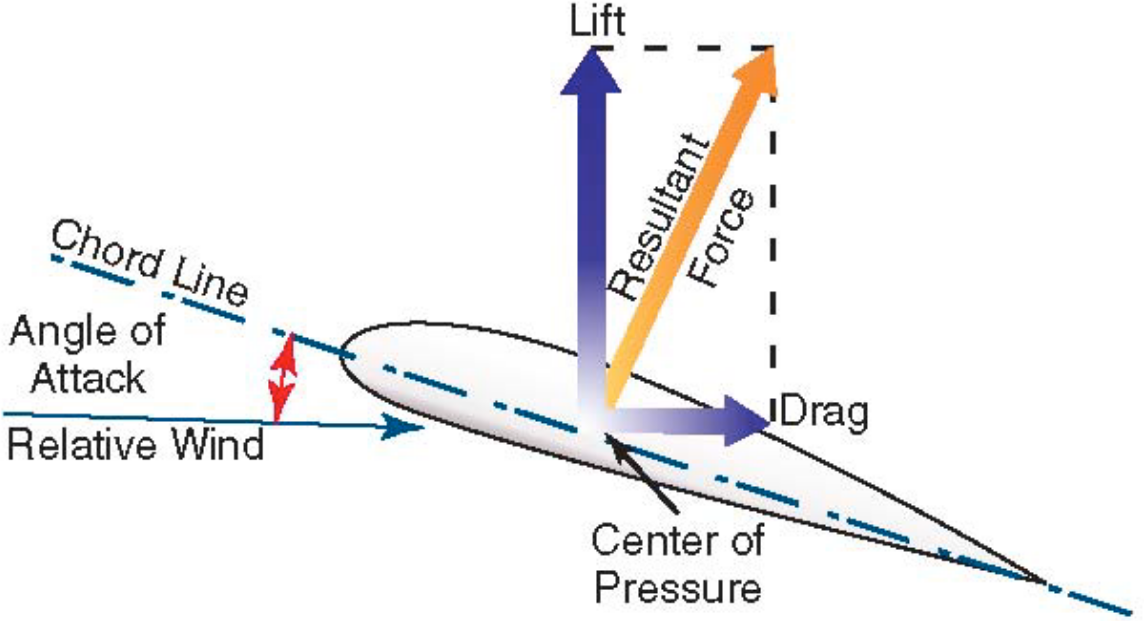
\includegraphics[width=.75\linewidth]{media/AOA.png}
\end{center}
\vfill \phantom{}
\newcolumn

\subsection{Angle of Incidence (AOI)}
Fixed angle between the chord line and the aircraft's
longitudinal axis; set during design and affects baseline performance
\begin{center}
  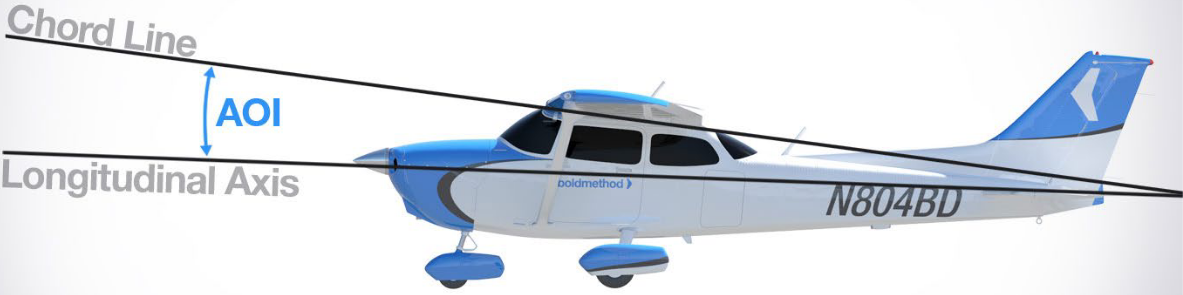
\includegraphics[width=.75\linewidth]{media/AOI.png}
\end{center}

\subsection{Center of pressure}
Centre of pressure is the resultant of the pressure distribution on
an airfoil
\begin{center}
  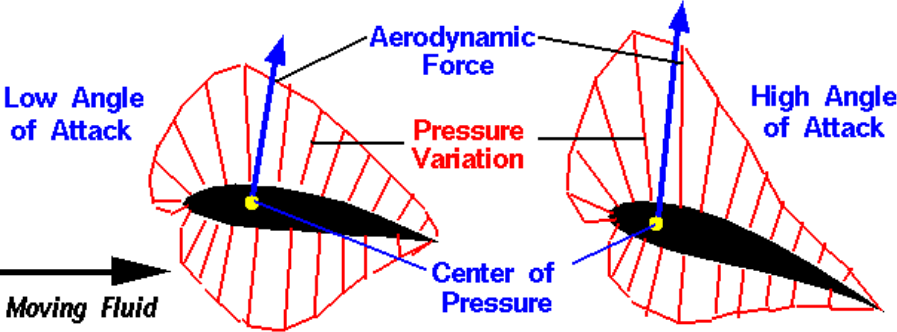
\includegraphics[width=.75\linewidth]{media/centerofpressure.png}
\end{center}

\subsection{NACA Series}
\subsubsection{4-Digit-Series}
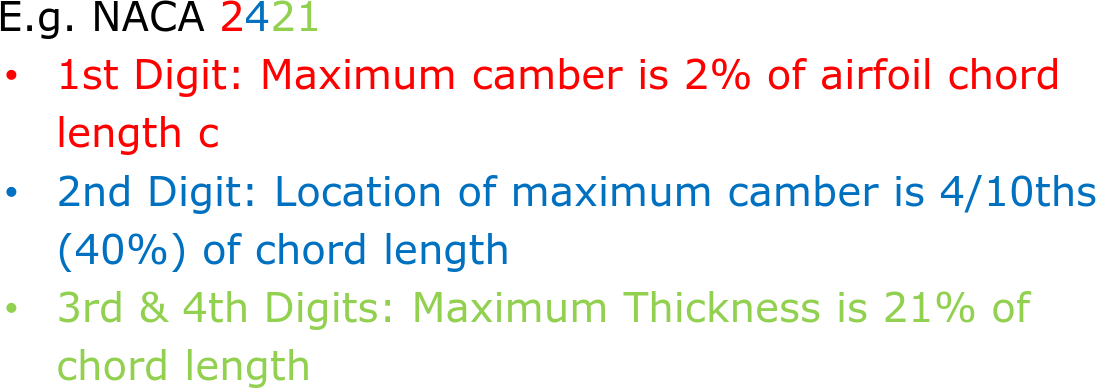
\includegraphics[width=.7\linewidth]{media/NACA4.png}

\subsubsection{5-Digit-Series}
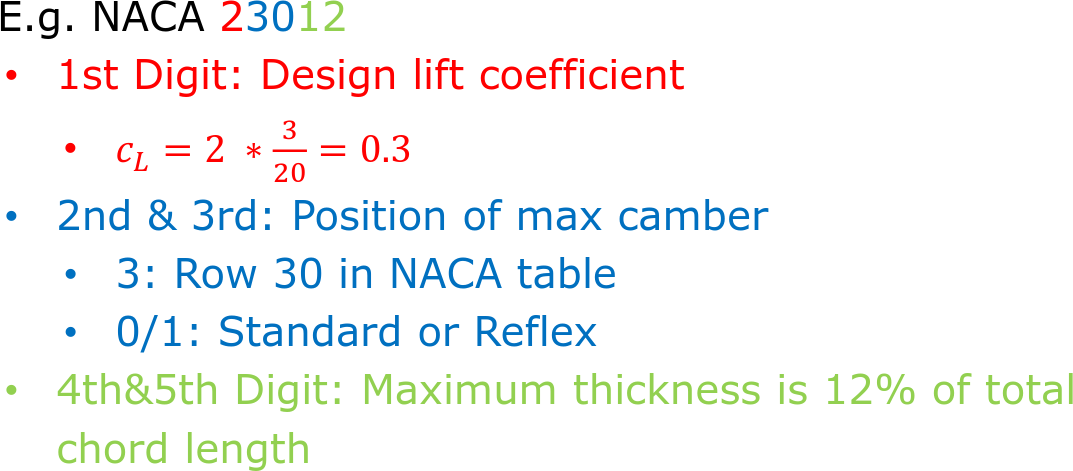
\includegraphics[width=.7\linewidth]{media/NACA5.png}

\section{Airfoil terminology}
\begin{center}
  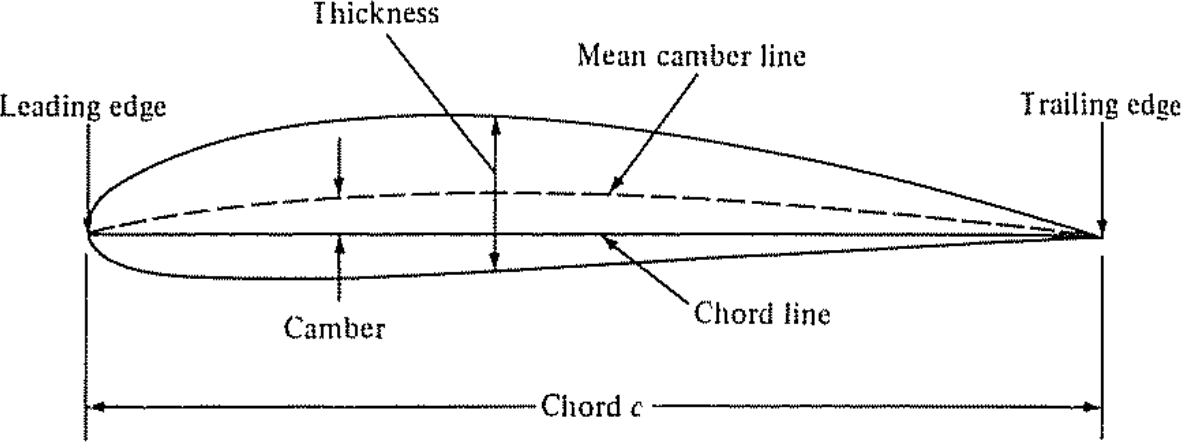
\includegraphics[width=.8\linewidth]{media/airfoil.png}
\end{center}
\vfill \phantom{}
\newcolumn

\vspace*{-.7cm}
\part{Dimensional Analysis and Similarity}
\section{Dimensional homogeneity}
\begin{center}
  \renewcommand{\arraystretch}{1.2}
  \begin{tabularx}{\linewidth}{|X|l|X|}
    \hline \textbf{Name} & \textbf{Variable} & \textbf{Primary Dimension} \\
    \hline Length & $l,d$ & $L$ \\
    \hline Time & $t$ & $T$ \\
    \hline Mass & $m$ & $M$ \\
    \hline Temperature & $T$ & $\Theta$ \\
    \hline Molar amount & $n$ & $N$ \\
    \hline Velocity & $u,v,w$ & $L\,T^{-1}$ \\
    \hline Rotational Speed & $s$ & $T^{-1}$ \\
    \hline Acceleration & $a,g$ & $L\,T^{-2}$ \\
    \hline Kinematic Viscosity & $\nu$ & $L^{2}T^{-1}$ \\
    \hline Diffusion coefficient & $D$ & $L^{2}T^{-1}$ \\
    \hline Force & $F$ & $L\,T^{-2}M$ \\
    \hline Energy & $E$ & $L^{2}T^{-2}M$ \\
    \hline Work, Heat & $W,Q$ & $L^{2}T^{-2}M$ \\
    \hline Power & $P$ & $L^{2}T^{-3}M$ \\
    \hline Pressure & $p$ & $L^{-1}T^{-2}M$ \\
    \hline Impuls & $I$ & $L\,T^{-1}M$ \\
    \hline Surface Tension & $\gamma,\sigma$ & $T^{-2}M$ \\
    \hline Density & $\rho$ & $L^{-3}M$ \\
    \hline Dynamic Viscosity & $\eta$ & $L^{-1}T^{-1}M$ \\
    \hline Heat Capacity & $C$ & $L^{2}T^{-2}M\Theta^{-1}$ \\
    \hline Molar heat capacity & $c$ & $L^{2}T^{-2}M\Theta^{-1}N^{-1}$ \\
    \hline
  \end{tabularx}
\end{center}

\section{Similarity}
Three basic laws of similarity must be satisfied in order to achieve complete similarity between prototype and
model flow fields
\subsection{Geometric similarity}
\begin{itemize}
  \item Model and prototype have same shape
  \item Linear dimensions on model and prototype correspond within constant scale factor
\end{itemize}
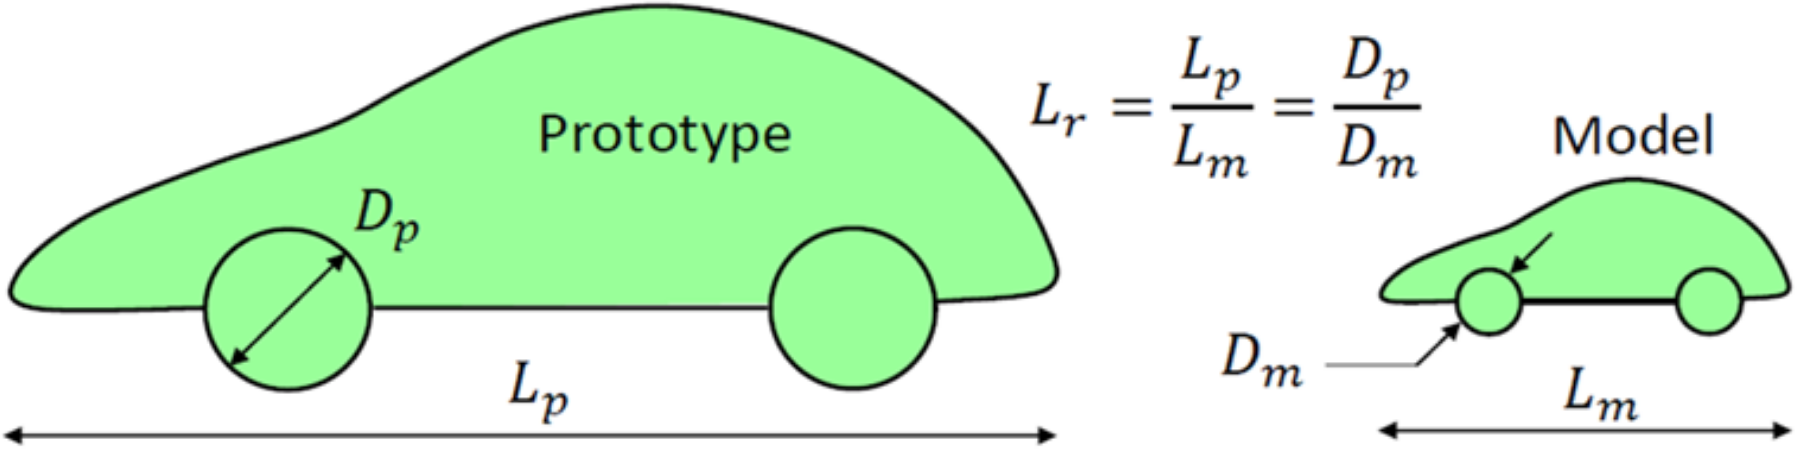
\includegraphics[width=\linewidth]{media/geometric.png}

\subsection{Kinematic similarity}
Velocities at corresponding points on model and prototype differ only by a constant scale factor
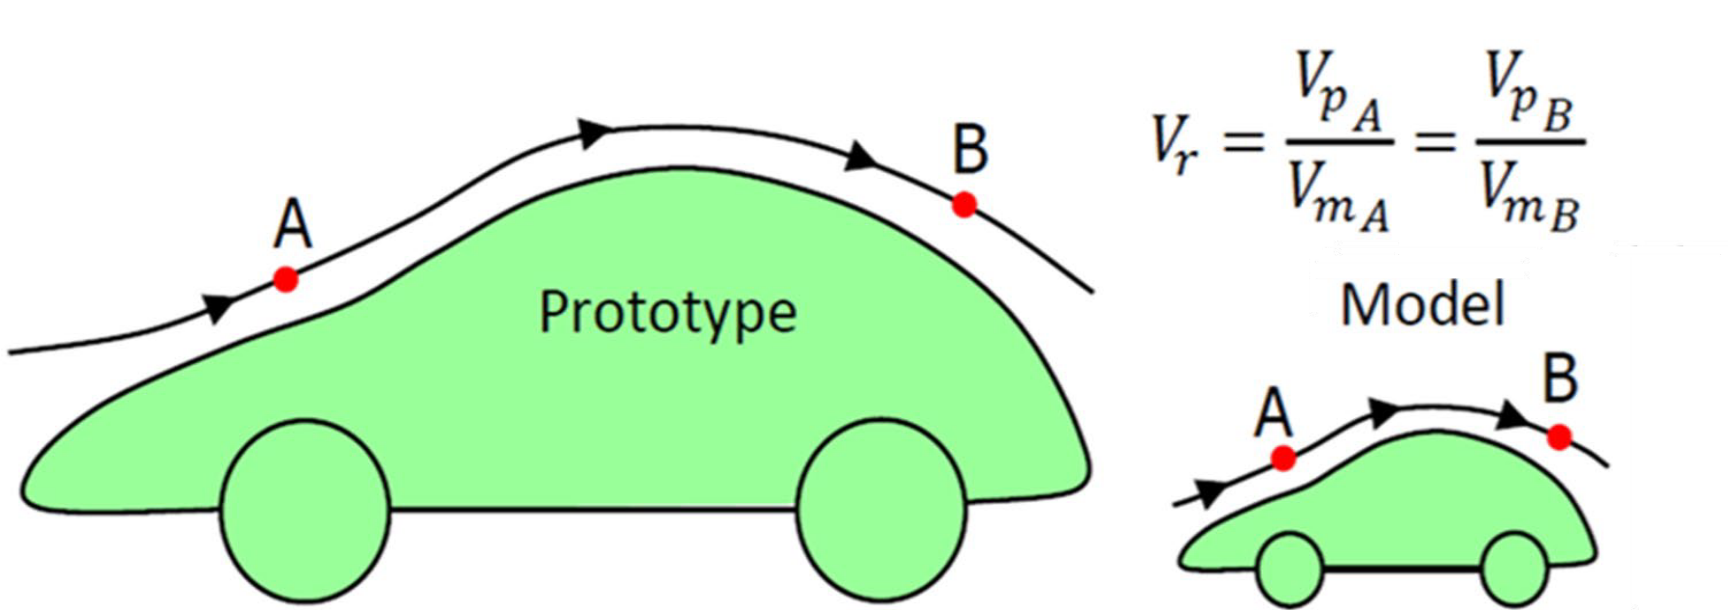
\includegraphics[width=\linewidth]{media/kinetic.png}

\subsection{Dynamic similarity}
All forces on model and prototype differ only by a constant scale factor

\section{Buckingham $\Pi$-Theorem}
Buckingham Pi-Theorem can be used to determine the nondimensional groups
of variables (Pi-Groups) for a given set of dimensional variables.

\begin{enumerate}[label=Step \arabic*.]
  \item List all the dimensional variables involved (n)
  \item Express each variables using primary dimensions (r):
    \begin{itemize}
      \item Only L: \textbf{geometric variables}
      \item Only T or both L and T: \textbf{kinematic variables}
      \item Those who have M: \textbf{dynamic variables}
    \end{itemize}
  \item Determine the repeating variables that are allowed to appear in more than one Pi-group
  \item Determine (n-r) many Pi-Groups by combining repeating variables with non-repeating variables and using the fact that Pi-Groups should be non-dimensional
\end{enumerate}

\subsection{Example with drag force}
\begin{center}
  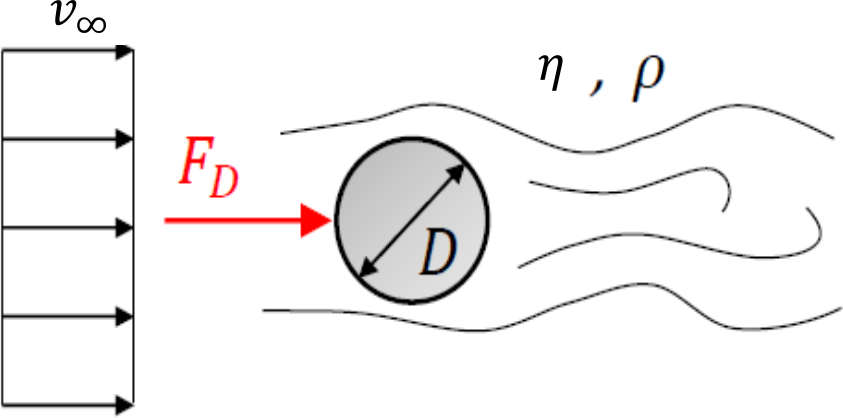
\includegraphics[width=.5\linewidth]{media/buckingham.png}
\end{center}

\begin{enumerate}[label=Step \arabic*.]
  \item $\dm n = \left(F_D, D, v_\infty, \eta, \rho\right) = 5$\\[0ex]
  \item $\dm F_D = \frac{ML}{T^2};\quad D = L;\quad v_\infty = \frac{L}{T};\quad \rho = \frac{M}{L^3};\quad \eta = \frac{M}{LT}$\\[0ex]
        $r = \left[D, v_\infty, \left(F_D, \eta, \rho\right)\right] = 3$\\[0ex]
  \item Repeating variables: $D\ [L], v_\infty\ [T], \rho\ [M]$\\[0ex]
  \item Number of $\Pi$-groups: $n-r = 5-3 = 2$\\[0.5ex]
        $\dm \Pi_1 = F_D D^{a_1} v_\infty^{b_1} \rho^{c_1}\quad ; \quad \Pi_2 = \eta D^{a_2} v_\infty^{b_2} \rho^{c_2}$
\end{enumerate}

\section{Nondimensional numbers}
\subsection{Euler Number}
\figbox{$\dm Eu = \frac{\text{Pressure energy}}{\text{Kinetic energy}} = \frac{\Delta p}{\rho v^2} = \frac{gH}{v^2}$}
Important for:
\vspace*{-.2cm}
\begin{itemize}
  \item Nozzle and Diffuser
  \item Pipe and Ducts
  \item Pumps and Turbines
\end{itemize}


\subsection{Grasshof Number}
\figbox{$\dm Gr = \frac{\text{Buoyancy force}}{\text{Viscous forces}} = \frac{L^3 g \beta \Delta T}{\nu}$}
Important for:
\vspace*{-.2cm}
\begin{itemize}
  \item \textbf{Natural (Free) Convection}
  \item $Gr \ll 1$: Conduction dominates
  \item $Gr \gg 1$: Convection dominates
  \item Radiators and heaters
  \item Cooling of electronics (no Fan)
\end{itemize}

\subsection{Froude Number}
\figbox{$\dm \frac{\text{Inertia forces}}{\text{Gravitational force}} = \frac{v}{\sqrt{gL}}$}
Important for:
\vspace*{-.2cm}
\begin{itemize}
  \item Ship Design: Controls wave formation and resistance
  \item General water flows
  \item Open channel / Free Surface flows
  \item $Fr \ll 1$: Gravity has high influence
  \item $Fr \gg 1$: Gravity negligible
\end{itemize}

\subsection{Cavitation Number}
\figbox{$\dm Ca = \sigma = \frac{p\infty-p_v}{\frac{1}{2}\rho v^2}$}
Important for:
\vspace*{-.2cm}
\begin{itemize}
  \item Pump Design, Ship Propeller Design
  \item Describes savety margin to cavitation:\\
  $\sigma \approx 1$: Pressure close to vapor pressure
\end{itemize}

\subsection{Weber Number}
\figbox{$\dm We = \frac{\text{Inertia forces}}{\text{Surface tension forces}} = \frac{\rho v L^2}{\sigma}$}
Important for:
\vspace*{-.2cm}
\begin{itemize}
  \item Fuel injection
  \item Jet breakup
  \item Bubble formation
\end{itemize}

\subsection{Prandlt Number}
\figbox{$\dm Pr = \frac{\text{Viscous diffusion}}{\text{Thermal diffusivity}} = \frac{c_p\nu}{\lambda} = \frac{\nu}{\alpha}$}
\begin{itemize}
  \item $Pr < 1$: Heat diffuses quickly compared to viscous (momentum) diffusion
  \item $Pr = 1$: Momentum BL $\sim$ Temperature BL
  \item $Pr > 1$: Heat is transported through diffusion in momentum
\end{itemize}

\subsection{Nusselt Number (Forced Convection)}
Nusselt number is to the thermal boundary layer what the friction coefficient is to the
velocity boundary layer:
\figbox{$\dm Nu = \frac{\alpha L}{\lambda} \approx \frac{\text{Convective heat transfer}}{\text{Conductive heat transfer}} = f(x^*, Re_L, Pr)$}
\begin{center}
  \footnotesize
  \setcellgapes{4pt}
  \makegapedcells
  \begin{tabular}{|l|c|c|c|}
    \hline
    \textbf{Regime} & \makecell[c]{\textbf{Velocity BL}} & \makecell[c]{\textbf{Thermal BL}} & $\bm{Nu(x)}$ \\
    \hline
    Laminar &
    $\dm \delta(x) = x \cdot \frac{4.91}{\sqrt{Re_x}}$ &
    $\dm \frac{\delta_t}{\delta} \approx Pr^{-1/3}$ &
    $\dm 0.332\,Re^{\frac{1}{2}}Pr^{0.7}$ \\
    \hline
    Turbulent &
    $\dm \delta(x) = x \cdot \frac{0.16}{Re_x^{1/7}}$ &
    $\dm \frac{\delta_t}{\delta} \approx Pr^{-1/3}$ &
    $\dm 0.023\,Re^{0.8}Pr^{1/3}$ \\
    \hline
  \end{tabular}
  \nomakegapedcells
\end{center}

\part{Potential flow}
\section{Irrotationality}
\begin{center}
  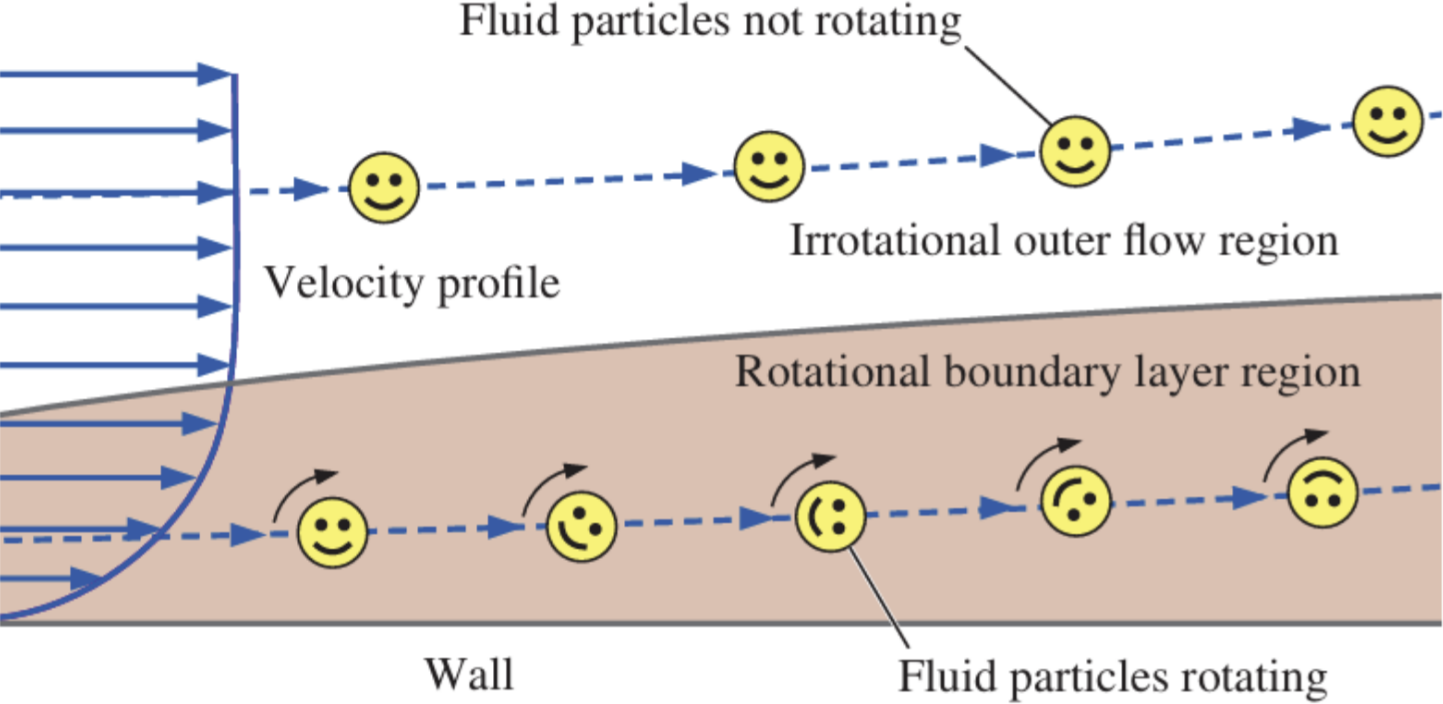
\includegraphics[width=.8\linewidth]{media/irrotationality.png}
  \[\tau = \eta\frac{du}{dy} = 0\]
\end{center}

\section{Vorticity}
\subsection{2D flow}
For fluids with constant viscosity, a 2D flow is irrotational when:
\begin{gather*}
  \dfrac{\partial v}{\partial x} = \dfrac{\partial u}{\partial y}\\
  \omega_z = \dfrac{\partial v}{\partial x} - \dfrac{\partial u}{\partial y} = 0
\end{gather*}

\subsection{3D flow}
In 3D, the velocity becomes a vector:
\begin{gather*}
  \underline{u} = \begin{pmatrix} u \\ v \\ w \end{pmatrix}\\
  \underline{\omega} = \rot(\underline{u}) = \nabla \times \underline{u} = \begin{pmatrix}
    0\\0\\0
  \end{pmatrix}
\end{gather*}

\subsubsection{Cartesian system}
\begin{equation*}
  \underline{u} =
  \begin{pmatrix}
    u\\
    v\\
    w
  \end{pmatrix}
  \text{ and }
  \nabla =
  \begin{pmatrix}
    \dfrac{\partial}{\partial x}\\[1.2ex]
    \dfrac{\partial}{\partial y}\\[1.2ex]
    \dfrac{\partial}{\partial z}
  \end{pmatrix} \Rightarrow
  \begin{pmatrix}
    \omega_x\\
    \omega_y\\
    \omega_z
  \end{pmatrix}
  =
  \begin{pmatrix}
    \dfrac{\partial w}{\partial y} - \dfrac{\partial v}{\partial z}\\[1.2ex]
    \dfrac{\partial u}{\partial z} - \dfrac{\partial w}{\partial x}\\[1.2ex]
    \dfrac{\partial v}{\partial x} - \dfrac{\partial u}{\partial y}
  \end{pmatrix}
\end{equation*}

\subsubsection{Cylindrical system}
\begin{equation*}
  \underline{u} =
  \begin{pmatrix}
    u_r\\
    u_\theta\\
    u_z
  \end{pmatrix}
  \text{ and }
  \nabla =
  \begin{pmatrix}
    \dfrac{\partial}{\partial r}\\[1.2ex]
    \dfrac{1}{r}\dfrac{\partial}{\partial \theta}\\[1.2ex]
    \dfrac{\partial}{\partial z}
  \end{pmatrix} \Rightarrow
  \begin{pmatrix}
    \omega_r\\
    \omega_\theta\\
    \omega_z
  \end{pmatrix}
  =
  \begin{pmatrix}
    \dfrac{1}{r}\dfrac{\partial u_z}{\partial \theta} - \dfrac{\partial u_\theta}{\partial z}\\[1.2ex]
    \dfrac{\partial u_r}{\partial z} - \dfrac{\partial u_z}{\partial r}\\[1.2ex]
    \dfrac{1}{r}\dfrac{\partial\left(r u_\theta\right)}{\partial r} - \dfrac{1}{r}\dfrac{\partial u_r}{\partial \theta}
  \end{pmatrix}
\end{equation*}

\section{Potential fields}
\begin{gather*}
  \rot(\underline{u}) =
  \begin{pmatrix}
    \omega_x \\ \omega_y \\ \omega_z
  \end{pmatrix}
  = 0\\
  \underline{u} = \nabla(\Phi) \Longrightarrow
  \begin{pmatrix}
    u\\v\\w
  \end{pmatrix}
  =
  \begin{pmatrix}
    \dfrac{\partial \Phi}{\partial x}\\[1.2ex]
    \dfrac{\partial \Phi}{\partial y}\\[1.2ex]
    \dfrac{\partial \Phi}{\partial z}
  \end{pmatrix}\\
  w_z = \dfrac{\partial^2\Phi}{\partial x \partial y} - \dfrac{\partial^2\Phi}{\partial y \partial x} = 0
\end{gather*}

\section{General fluid motion}
\subsection{Governing equations}
\subsubsection{Continuity equation}
\[\frac{\partial \rho}{\partial t} + \nabla \cdot \rho \underline{u} = 0\]

\subsubsection{Momentum equation}
\[\frac{\partial \rho\underline{u}}{\partial t} + \nabla\cdot \rho\underline{u}\ \underline{u} = \nabla p +\eta\nabla \cdot \underline{\underline{\tau}}\]

\newcolumn
\subsection{Simplifications}
\begin{itemize}
  \item Inviscid: $\eta = 0$
  \item Steady: $\dfrac{\partial}{\partial t} = 0$
  \item Irrotational: $\rot(\underline{u})=0 \to \underline{u} = \nabla\Phi$
  \item Incompressible: $\rho=\const$
  \item Continuity: $\nabla\cdot\underline{u} = 0$ 
\end{itemize}

\subsection{Potential flow model}
\begin{itemize}
  \item Velocity potential: $\underline{u} = \nabla\Phi$
  \item Laplace governing equation: $\nabla^2\Phi = 0$
  \item Pressure field (Euler $\to$\ Bernoulli): $p+\frac{1}{2}\rho u^2 = \const$
\end{itemize}

\section{Potential function $\phi(x,y)$}
\subsection{Scalar potential field and Potential flow}
Incompressible, steady flow and irrotational:
\[\zeta = \rot(u) = \nabla \times u = 0\]
Hence:
\[u = \nabla\Phi = \begin{pmatrix}
  u\\v
\end{pmatrix} =
\begin{pmatrix}
  \frac{\nabla \Phi}{\partial x}\\[1.2ex]
  \frac{\nabla \Phi}{\partial y}
\end{pmatrix}\]

\subsection{Continuity equation}
\[\nabla \cdot u = 0 \to \nabla\cdot\nabla\Phi = \nabla^2\Phi = 0\]

\subsection{Momentum (Euler) equation}
\[u\cdot\nabla u = \nabla\frac{1}{2}\left|u\right|^2u \cdot \nabla u = \nabla\frac{1}{2}\left|u\right|^2-u\times(\nabla\times u)\]
which reduces to:
\[\nabla\frac{1}{2}\left|u\right|^2+\frac{p}{\rho}=\const\]

\section{Stream function $\psi(x,y)$}
Incompressible, steady flow:
\[u = \frac{\partial\psi}{\partial y} = \frac{\partial\Phi}{\partial x}\quad \text{and}\quad v = -\frac{\partial \psi}{\partial x} = \frac{\partial\Phi}{\partial y}\]
For $\nabla\cdot u = 0$:
\[\nabla \cdot u = \frac{\partial u}{\partial x} + \frac{\partial v}{\partial y} = \frac{\partial^2}{\partial x \partial y} - \frac{\partial^2 \psi}{\partial y \partial x} = 0\]























\end{multicols*}

\end{document}
